\chapter{building tempest 2000 in 1994}
\label{sec:building_t2k}
\lstset{style=68KStyle}
\lhead[tempest 2000]{}

It is 1994 and Atari have asked you create the flagship launch title for their new video game console,
the Atari Jaguar. No need to come to Sunnyvale in California, you can stay in your valley in Wales and
let us know when you're finished.

\begin{figure}[H]
      \centering
      \frame{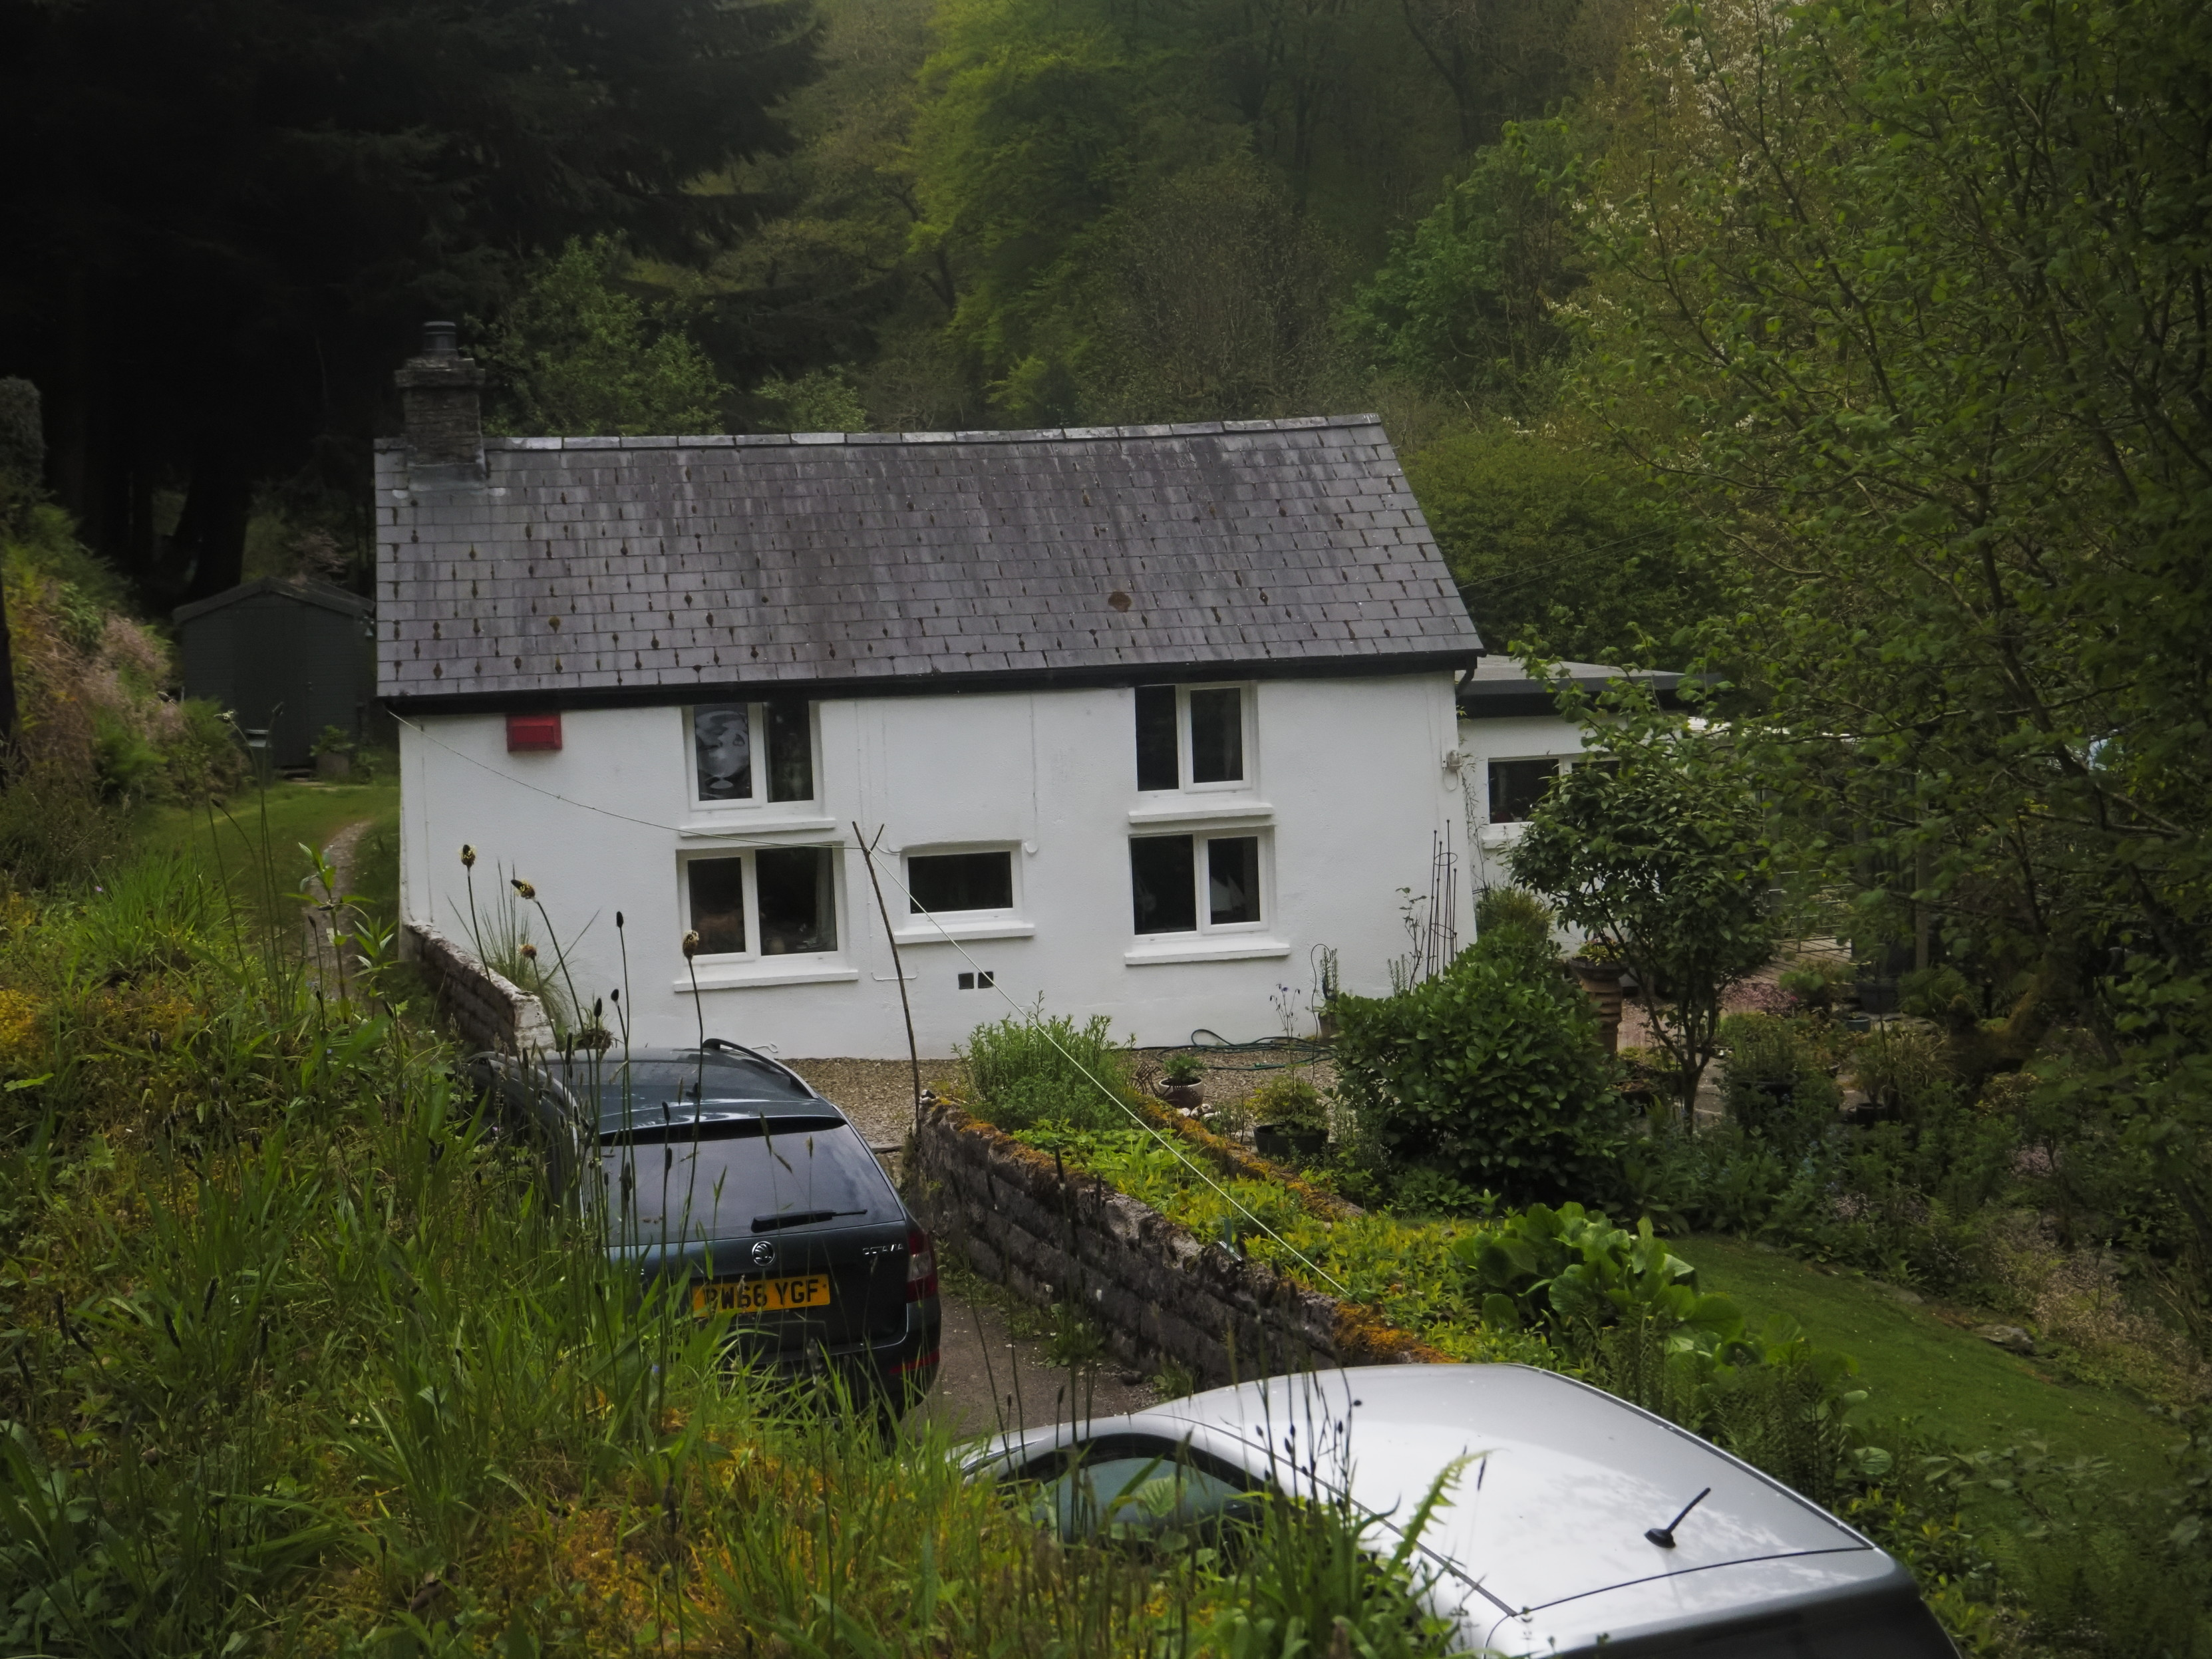
\includegraphics[width=8cm]{src/build_t2k/cwmcych.jpg}}%
    \caption{You are not in California, you are in Cwmcych in Wales and that's where you'll make Tempest 2000.}
\end{figure}

So instead of sitting two doors down from the computer room armed with just a pencil, you are instead 
expected to conjure a game that will launch a machine on which the future of Atari depends from your cottage.
To get you started you will be sent a console and a manual. You already have a computer we assume.

So because it's the way you've always done it, you get started writing \icode{Tempest 2000} in one big file
of Motoral 68K assembly code.
And because you always get to name things whatever you want, you name this file \icode{YAK.S}, because that's the 
the three-letter name you use on high score tables.

\begin{figure}[H]
      \centering
      \frame{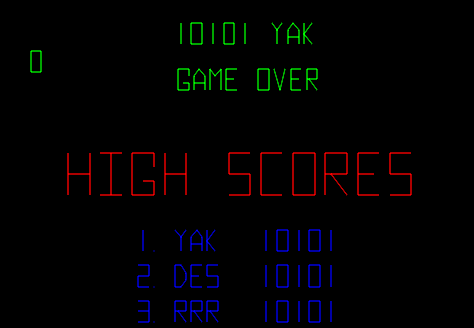
\includegraphics[width=8cm]{src/build_t2k/yak.png}}%
    \caption{YAK has the top score in Tempest.}
\end{figure}

Assembling this code will be a simple matter of running the \icode{madmac} assembler as follows:

\begin{lstlisting}
$mac -fb -isrc -l src/yak.s -o yak.dat
\end{lstlisting}

We're not done yet though.
In addition to a cryptic name for the main megafile (\icode{YAK.S} will eventually run to almost 20,000
lines of code), we also need to write a bunch of programs in a custom flavour of 68K Motorola assembly for
the Jaguar's GPU. These programs will handle all the hard mathematics for generating polygons in three
dimensions. Because no-one else will ever need to read this code we can name them whatever we want. So
we'll continue the zoological theme and name them after more beasts of the field. There will be nine GPU
programs in total, each doing something specific (for example, scaling and rotating objects in \icode{antelope.gas}) 
and some of them doing the same things but slightly differently (variations of a Robotron-style particle
explosion in \icode{camel.gas} and \icode{xcamel.gas}).

This is roughly what it looks like when we assemble each of our GPU programs.
\begin{lstlisting}
$ mac -fr -mtom -l -isrc donky.gas -o donky.dat
$ mac -fr -mtom -l -isrc camel.gas -o camel.dat
$ mac -fr -mtom -l -isrc antelope.gas -o antelope.dat
$ mac -fr -mtom -l -isrc goat.gas -o goat.dat
$ mac -fr -mtom -l -isrc llama.gas -o llama.dat
$ mac -fr -mtom -l -isrc horse.gas -o horse.dat
$ mac -fr -mtom -l -isrc ox.gas -o ox.dat
$ mac -fr -mtom -l -isrc stoat.gas -o stoat.dat
$ mac -fr -mtom -l -isrc xcamel.gas -o xcamel.dat
\end{lstlisting}

Now is a good time to be dealing with less objects, so let's create another file called \icode{YAKGPU.S} that
collates all our GPU programs into one big GPU object. Here's how we do that in \icode{YAKGPU.S}:

\begin{lstlisting}
;
;	CONSTANT DATA (GPU PROGRAMS)
;
fastvector:
	.include	"llama.dat"
xvector:
	.include 	"goat.dat"
demons:
	.include	"antelope.dat"
parrot:
	.include	"camel.dat"
xparrot:
	.include	"xcamel.dat"
texter:
	.include 	"stoat.dat"
bovine:
	.include	"ox.dat"
equine:
	.include 	"horse.dat"
equine2:
	.include 	"donky.dat"
\end{lstlisting}

And here's how we assemble \icode{YAKGPU.S}:
\begin{lstlisting}
$ mac -fb -isrc yakgpu.s -o yakgpu.dat
\end{lstlisting}

We have one more object file to pull together. An omnibus containing all our image and sound data. For this
we will create a file called \icode{IMAGES\_SOUNDS.S}. At the top we will put all our image files:

\begin{lstlisting}
.incbin "beasty3.cry"
.incbin "beasty4.cry"
.incbin "beasty5.cry"
.incbin "beasty6.cry"
.incbin "beasty7.cry"
.incbin "beasty8.cry"
\end{lstlisting}

We are still in a proverbial farmyard with our naming conventions. Let's take a look at what's actually in these files:

\begin{figure}[H]
  {
    \setlength{\tabcolsep}{3.0pt}
    \setlength\cmidrulewidth{\heavyrulewidth} % Make cmidrule = 
    \begin{adjustbox}{width=10cm,center}

      \begin{tabular}{ll}
        \toprule
        \tcode{beasty3.cry} &\tcode{beasty4.cry} \\
        \midrule
        \makecell[l]{
            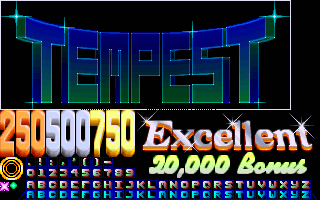
\includegraphics[width=2.2cm]{cry/beasty3.png} \\
        }
        &
        \makecell[l]{
            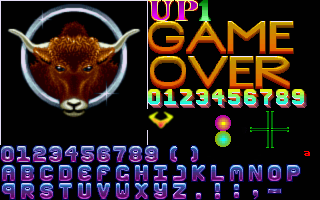
\includegraphics[width=2.2cm]{cry/beasty4.png} \\
        }
       \\ 
        \toprule
        \tcode{beasty5.cry} &\tcode{beasty6.cry} \\
        \midrule
        \makecell[l]{
            
\includegraphics[width=2.2cm]{cry/beasty5.png} \\
        }
        &
        \makecell[l]{
            
\includegraphics[width=2.2cm]{cry/beasty6.png} \\
        }
       \\ 
        \toprule
        \tcode{beasty7.cry} &\tcode{beasty8.cry} \\
        \midrule
        \makecell[l]{
            
\includegraphics[width=2.2cm]{cry/beasty7.png} \\
        }
        &
        \makecell[l]{
            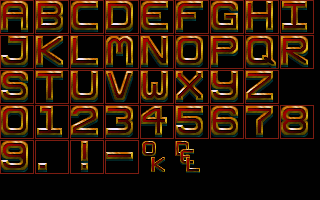
\includegraphics[width=2.2cm]{cry/beasty8.png} \\
        }
       \\ 
        \bottomrule
      \end{tabular}
    \end{adjustbox}
  }\caption*{The contents of our 'beasty' files.}
\end{figure}

Apart from attractive image data we also have some music to play. There are seven tunes for us to
include. These are:

\begin{lstlisting}
.incbin "sounds/tune13.mod"
.DC.L $0000
.incbin "sounds/tune7.mod"
.DC.L $0000
.incbin "sounds/tune1.mod"
.DC.L $0000
.incbin "sounds/tune3.mod"
.DC.L $0000
.incbin "sounds/rave4.mod"
.DC.L $0000
.incbin "sounds/tune5.mod"
.DC.L $0000
.incbin "sounds/tune12.mod"
.DC.L $0000
\end{lstlisting}

We also have a whole bunch of sound effects. But we'll get into those later. For now, let's assemble
our audiovisual bag of tricks into a single object file:
\begin{lstlisting}
$ mac -fb -isrc images_sounds.s -o images_sounds.dat
\end{lstlisting}

This leaves us with just one final step to perform: linking all of our products, \icode{YAK.DAT}, \icode{IMAGES\_SOUNDS.DAT},
and \icode{YAKGPU.DAT} together to give us a game we can actually play. For that we use Atari's purpose built 
linker \icode{aln}:

\begin{lstlisting}
$ aln -z -e -a 802000 4000 efa8 yak.dat vidinit.dat yakgpu.dat images_sounds.dat -o t2000.abs
\end{lstlisting}


